% !TeX root = construct.tex
\chapter{Mascheroni's Compass Problem}\label{c.compass-only}


\begin{quote}
This document is Problem $33$ from the book by Heinrich D\"{o}rrie: \textit{100 Problems of Elementary Mathematics: Their History and Solution} (Dover, 1965), as reworked by Michael Woltermann.\footnote{\url{http://www2.washjeff.edu/users/mwoltermann/Dorrie/DorrieContents.htm}. I would like to thank him for giving me permission to use his work.} I have added explanations so that students and teachers can better understand the construction. The document has been written and formatted in \LaTeX{}, and I have redrawn the diagrams using Ti\textit{k}Z, adding auxiliary lines and  drawing diagrams incrementally for clarity.

Moti Ben-Ari\footnote{\url{http://www.weizmann.ac.il/sci-tea/benari/}.}\\
Department of Science Teaching\\
Weizmann Institute of Science
\end{quote}

\bigskip

%%%%%%%%%%%%%%%%%%%%%%%%%%%%%%%%%%%%%%%%%%%%%%%%%%%%%%%%%%%%%%%

Prove that any construction that can be carried out with a compass and straight-edge can be carried out with the compass alone. The Italian L. Mascheroni (1750-1800) posed this problem to himself and solved it in a masterly fashion in his book \textit{La geometria del compasso}, published in Pavia in 1797.

\begin{quote}
The theorem is currently known as the Mohr-Mascheroni Theorem since it had been proved in 1672 by the Danish mathematician Georg Mohr, but his work was not widely known until the twentieth century.\footnote{A different proof can be found in: Norbert Hungerb\"{u}hler. A short elementary proof of the Mohr-Mascheroni theorem. \textit{American Mathematical Monthly} 101(8), 1994, 784--787.}
\end{quote}

When we examine the separate steps by which circle and straight-edge constructions are carried out, we see that every step consists of one of the following three basic constructions:

I. Finding the point of intersection of two straight lines;

II. finding the point of intersection of a straight line and a circle;

III. finding the point(s) of intersection of two circles.

Thus we need only show that the two basic constructions I. and II. can be done with a compass alone. (Mascheroni regarded a straight line as given if two of its points are known.)

First we will solve four preliminary problems. (Dörrie talks about two, but the others are embedded in these.) In the following:
\begin{itemize}
\item $C(O,A)$ stands for the circle with center $O$ through point $A$,
\item $C(O,AB)$ stands for the circle with center $O$ and radius $AB$.
\end{itemize}

%%%%%%%%%%%%%%%%%%%%%%%%%%%%%%%%%%%%%%%%%%%%%%%%%%%%%%%%%%%%%%%

\pagebreak[3]

\textbf{Prelim 1.} Reflect a point $C$ about the line through $A$ and $B$.

\begin{quote}
Given a point $C$ and a line $AB$, a reflection of $C$ about $AB$ is a point $C'$ such that $AB$ is the perpendicular bisector of the line $CC'$.
\end{quote}

\textbf{Solution.} The reflection $C'=c(A,C) \cap c(B,C)$ (not $C$ in general):

\begin{quote}
The phrase ``not $C$ in general'' rules out the possibility that $C$ is on the line containing $AB$, in which case there is nothing to do.
\end{quote}

\begin{center}
\begin{tikzpicture}[scale=.65]
\coordinate (A) at (0,0);
\coordinate (B) at (4,0);
\coordinate (C) at (2.5,1.5);
\draw[thick,dashed] ($(B)!2!(A)$) -- ($(A)!2!(B)$);
\fill (A) node[above left] {$A$} circle[radius=2pt];
\fill (B) node[above right] {$B$} circle[radius=2pt];
\fill (C) node[above,yshift=4pt] {$C$} circle[radius=2pt];
\node[draw,circle through=(C),name path=ac] at (A) {};
\node[draw,circle through=(C),name path=bc] at (B) {};
\path [name intersections={of=ac and bc,by={x1,Cp}}];
\fill (Cp) node[below,yshift=-4pt] {$C'$} circle[radius=2pt];
\draw (C) -- (Cp);
\draw[thick,dashed] (A) -- (C);
\draw[thick,dashed] (B) -- (C);
\draw[thick,dashed] (A) -- (Cp);
\draw[thick,dashed] (B) -- (Cp);
\end{tikzpicture}

Line $AB$ is the perpendicular bisector of chord $CC'$ of both circles
\end{center}

Note: Dashed lines in figures are drawn to explain the arguments, but are not used in constructions.  
\begin{quote}
The lines drawn in the diagrams serve \emph{only} to illustrate the proofs. You must convince yourself that a compass alone is used in all the constructions.

Proof that $C'$ is the reflection of $C$: $\triangle ABC$ and $\triangle ABC'$ are congruent by side-side-side since $AC,AC'$ are radii of the same circle as are $BC,BC'$, and $AB$ is a common side. Therefore, $\angle CAB = \angle C'AB$ so $AB$ is the angle bisector of $\angle CAC'$. Since $\triangle CAC'$ is an isosceles triangle, the angle bisector $AB$ is also the perpendicular bisector of the base of the triangle $CC'$, and by definition $C'$ is the reflection of $C$ around $AB$.
\end{quote}

%%%%%%%%%%%%%%%%%%%%%%%%%%%%%%%%%%%%%%%%%%%%%%%%%%%%%%%%%%%%%%%

\textbf{Prelim 2.} Construct $c(A,BC)$, given points $A,B,C$.

\begin{quote}
You might ask yourself why this is a problem. Simply place the two legs of the compass on $B$ and $C$, and then move the compass so that one leg is on $A$ and draw the circle which will have radius $BC$. The reason is that the compass used by Euclid is a ``collapsing'' compass whose legs cannot maintain a distance when the compass is raised off the paper. Euclid proved what is now called the ``Compass Equivalence Theorem'': any construction with a fixed compass can be done with a collapsing compass. If effect, Prelim. 2 is a proof of this theorem that uses only a compass.
\end{quote}

\textbf{Solution.} Let $X$ and $Y$ be the points of intersection of $c(A,B)$ and $c(B,A)$:

\begin{center}
\begin{tikzpicture}[scale=.55]
\coordinate (A) at (0,1.5);
\coordinate (B) at (0,-1.5);
\coordinate (C) at (1.5,-3);
\coordinate (Cp) at (1.5,3);
\fill (A) node[above] {$A$} circle[radius=3pt];
\fill (B) node[below] {$B$} circle[radius=3pt];
\fill (C) node[below] {$C$} circle[radius=3pt];
%\fill (Cp) node[above] {$C'$} circle[radius=3pt];
\node[draw,circle through=(B),name path=ab] at (A) {};
\node[draw,circle through=(A),name path=ba] at (B) {};
\path [name intersections={of=ab and ba,by={Y,X}}];
\fill (X) node[above right,xshift=4pt] {$X$} circle[radius=3pt];
\fill (Y) node[above left,xshift=-4pt] {$Y$} circle[radius=3pt];
\draw[thick,dashed] ($(X)!2.3!(Y)$) -- ($(Y)!2!(X)$);
\end{tikzpicture}
\vspace*{-6pt}
\end{center}

Let $C'$ be the reflection of $C$ about line $XY$:

\begin{quote}
\vspace*{-6pt}
By Prelim. 1, this construction can be done using only a compass.
\end{quote}

\begin{center}
\vspace*{-6pt}
\begin{tikzpicture}[scale=.45]
\coordinate (A) at (0,1.5);
\coordinate (B) at (0,-1.5);
\coordinate (C) at (1.5,-3);
\coordinate (Cp) at (1.5,3);
\fill (A) node[right] {$A$} circle[radius=3pt];
\fill (B) node[right] {$B$} circle[radius=3pt];
\fill (C) node[below,yshift=-2pt] {$C$} circle[radius=3pt];
\fill (Cp) node[above,xshift=2pt,yshift=2pt] {$C'$} circle[radius=3pt];
\node[circle through=(B),name path=ab] at (A) {};
\node[circle through=(A),name path=ba] at (B) {};
\path [name intersections={of=ab and ba,by={Y,X}}];
\fill (X) node[above right,xshift=4pt] {$X$} circle[radius=3pt];
\fill (Y) node[above left,xshift=-4pt] {$Y$} circle[radius=3pt];
\node[draw,circle through=(C)] at (X) {};
\node[draw,circle through=(C)] at (Y) {};
\draw[thick,dashed] ($(X)!2.3!(Y)$) -- ($(Y)!2!(X)$);
%\draw (X) -- (Y) -- (C) -- (X) -- (Cp) -- (Y);
\draw[thick,dashed] (C) -- (Cp);
\end{tikzpicture}
\vspace*{-6pt}
\end{center}

$c(A,C')$ is the desired circle:

\begin{center}
\begin{tikzpicture}[scale=.5]
\coordinate (A) at (0,1.5);
\coordinate (B) at (0,-1.5);
\coordinate (C) at (1.5,-3);
\coordinate (Cp) at (1.5,3);
\fill (A) node[above,yshift=2pt] {$A$} circle[radius=3pt];
\fill (B) node[below,yshift=-2pt] {$B$} circle[radius=3pt];
\fill (C) node[below,yshift=-2pt] {$C$} circle[radius=3pt];
\fill (Cp) node[above,yshift=2pt] {$C'$} circle[radius=3pt];
\node[circle through=(B),name path=ab] at (A) {};
\node[circle through=(A),name path=ba] at (B) {};
\path [name intersections={of=ab and ba,by={Y,X}}];
\fill (X) node[above right,xshift=4pt] {$X$} circle[radius=3pt];
\fill (Y) node[above left,xshift=-4pt] {$Y$} circle[radius=3pt];
\node[circle through=(C)] at (X) {};
\node[draw,circle through=(C)] at (Y) {};
\draw[thick,dashed] ($(X)!2.3!(Y)$) -- ($(Y)!2!(X)$);
\path[name path=xy] (X) -- (Y);
\node[draw,thick,circle through=(Cp)] at (A) {};
\draw[very thick] (A) -- (Cp);
\draw[very thick] (B) -- (C);
\draw[very thick,name path=abline] (A) -- (B);
\draw[very thick,name path=ccp] (C) -- (Cp);
\path [name intersections={of=xy and abline,by={D}}];
\path [name intersections={of=xy and ccp,by={E}}];
\fill (D) node[above left] {$D$} circle[radius=3pt];
\fill (E) node[below right] {$E$} circle[radius=3pt];
\draw[thick,dashed] (D) -- (Cp);
\draw[thick,dashed] (D) -- (C);
\end{tikzpicture}
\vspace*{-4pt}
\end{center}

Since $A$ is the reflection of $B$ about $XY$, and reflection preserves distance, so $AC'=BC$.

\begin{quote}
$A$ is the reflection of $B$ around $XY$, and $C'$ is the reflection of $C$ around the $XY$. By definition $XY$ is the perpendicular bisector of $CC'$ and $AB$, so $C'E=EC$, $AD=DB$ and $\angle DEC=\angle DEC'(=90^\circ)$. $\triangle DEC$ is congruent to $\triangle DEC'$ by side-angle-side, so $DC=DC'$ and $\angle ADC'=\angle BDC$ (they are complementary to $\angle C'DE$, $\angle CDE$). Therefore, $\triangle ADC'$ is congruent to $\triangle BDC$, so $AC'=BC$.
\end{quote}

%%%%%%%%%%%%%%%%%%%%%%%%%%%%%%%%%%%%%%%%%%%%%%%%%%%%%%%%%%%%%%%

\textbf{Prelim 3.} Construct the sum or difference of two given segments $a$ and $b$, i.e., lengthen or shorten a given segment $PQ = a$ by a segment $QX = b$. (See Prelim 2 if necessary to construct a segment of length $b$ at $Q$.)

\begin{quote}
This would be trivial if we had a straight-edge. Simply extend the line segment $PQ$ of length $a$ with the straight-edge, copy line segment $RS$ of length $b$ so that $Q$ is one end point and construct a circle of radius $b$. The intersections of the circle with the ray give the required line segments $PU$ of length $a-b$ and $PT$ of length $a+b$:
\begin{center}
\vspace*{-2ex}
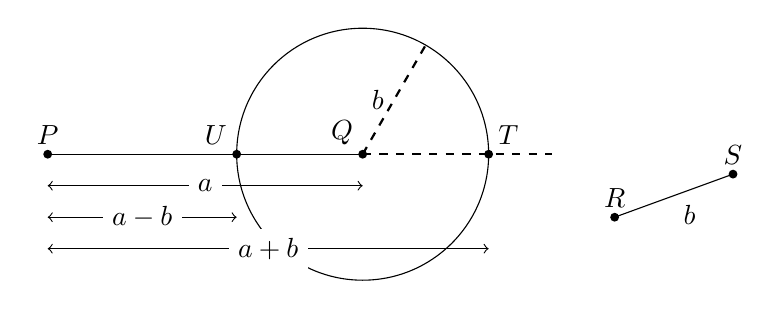
\begin{tikzpicture}[scale=.8]
\draw (0,0) -- (5,0);
\fill (0,0) node[above] {$P$} circle[radius=2pt];
\fill (5,0) node[above left] {$Q$} circle[radius=2pt];
\fill (3,0) node[above left] {$U$} circle[radius=2pt];
\fill (7,0) node[above right] {$T$} circle[radius=2pt];
\draw[thick,dashed] (5,0) -- (8,0);
\draw (5,0) circle[radius=2cm];
\draw[thick,dashed] (5,0) -- node[left] {$b$} ++(60:2cm);
\draw (9,-1) node[above] {$R$} -- node[below right] {$b$} ++(20:2cm) node[above] {$S$};
\fill (9,-1) circle[radius=2pt];
\fill (9,-1) ++(20:2cm) circle[radius=2pt];
\draw[<->] (0,-.5) -- node[fill=white] {$a$} (5,-.5);
\draw[<->] (0,-1) -- node[fill=white] {$a-b$} (3,-1);
\draw[<->] (0,-1.5) -- node[fill=white] {$a+b$} (7,-1.5);
\end{tikzpicture}
\end{center}
\vspace*{-4ex}
\end{quote}

\textbf{Solution.}

1. Let $H$ be any point on $c(Q,b)$, and $H'$ its reflection about line $PQ$. Let $h$ be the (length of) segment $HH'$:
\begin{center}
\begin{tikzpicture}[scale=.6]
\coordinate (Q) at (0,0);
\coordinate (P) at (-6.8,0);
\coordinate (B) at (-3,-2);
\draw[thick,dashed] ($(Q)!1.3!(P)$) -- node[above,near start] {$a$} ($(P)!2.3!(Q)$);
\fill (Q) node[above left] {$Q$} circle[radius=2pt];
\fill (P) node[above] {$P$} circle[radius=2pt];
\fill (B) circle[radius=2pt];
\node[draw,circle through=(B),name path=qb] at (Q) {};
\draw[thick,dashed] (Q) -- node[left,xshift=-1pt,yshift=2pt] {$b$} (B);
\path[name path=qh] (Q) -- (-40:5cm);
\path[name path=qhp] (Q) -- (40:5cm);
\path [name intersections={of=qb and qh,by={H}}];
\path [name intersections={of=qb and qhp,by={Hp}}];
\fill[below right] (H) node[right,xshift=2pt] {$H$} circle[radius=2pt];
\fill[above right] (Hp) node[right,xshift=2pt] {$H'$} circle[radius=2pt];
\draw[thick,dashed] (H) -- node[below left,yshift=-2pt] {$h$} (Hp);
\end{tikzpicture}
\end{center}

2. Let $K = c(Q,h) \cap c(H,b)$ and $K'$ be the reflection of $K$ about line $PQ$:

\begin{center}
\begin{tikzpicture}[scale=.55]
\coordinate (Q) at (0,0);
\coordinate (P) at (-6.8,0);
\coordinate (B) at (-3,-2);
\draw[thick,dashed] ($(Q)!1.3!(P)$) -- ($(P)!2.3!(Q)$);
\fill (Q) node[above right] {$Q$} circle[radius=3pt];
\fill (P) node[above] {$P$} circle[radius=3pt];
\fill (B) circle[radius=3pt];
\node[draw,circle through=(B),name path=qb] at (Q) {};
\draw[thick,dashed] (Q) -- node[left,xshift=-1pt,yshift=2pt] {$b$} (B);
\path[name path=qh] (Q) -- (-40:5cm);
\path[name path=qhp] (Q) -- (40:5cm);
\path [name intersections={of=qb and qh,by={Hp}}];
\path [name intersections={of=qb and qhp,by={H}}];
\fill (H) node[right,xshift=2pt] {$H$} circle[radius=3pt];
\fill (Hp) node[right,xshift=2pt] {$H'$} circle[radius=3pt];
\draw (H) -- node[below left,yshift=-3pt] {$h$} (Hp);
\draw[thick,name path=circleqh] (Q) let
  \p1 = ($ (H) - (Hp) $),
  \n2 = {veclen(\x1,\y1)}
in
  circle (\n2)
  (Q) edge [dashed] node[below] {$h$} +(140:\n2) ++(140:\n2) coordinate (q);
\fill (q) circle[radius=3pt];
\draw[thick,name path=circlehb] (H) let
  \p1 = ($ (Q) - (B) $),
  \n2 = {veclen(\x1,\y1)}
in
  circle (\n2)
  (H) edge [dashed] node[below,near end] {$b$} +(50:\n2) ++(50:\n2)  coordinate (h);
\fill (h) circle[radius=3pt];
\path [name intersections={of=circleqh and circlehb,by={K}}];
\fill (K) node[above left] {$K$} circle[radius=3pt];
%\draw[thick] (H) -- (K);
\draw let
  \p1 = ($ (K) - (Q) $)
in
  coordinate (Kp) at (\x1,-\y1);
\fill (Kp) node[below left] {$K'$} circle[radius=3pt];
\draw (K) -- (Kp);
\end{tikzpicture}
\vspace*{-8pt}
\end{center}

Then $KHH'K'$ is an isosceles trapezoid with legs $KH = K'H' = b$ and base $KK' = 2h$. Let $d = KH' = K'H$:

\begin{quote}
We also have $h=HH'$ since $H'$ is a reflection of $H$. Since $K'$ is a reflection of $K$ and reflections preserve distance, $KH=K'H'$, defined to be $d$.
\end{quote}

\begin{center}
\vspace*{-8pt}
\begin{tikzpicture}[scale=.6]
\coordinate (Q) at (0,0);
\coordinate (P) at (-6.8,0);
\coordinate (B) at (-3,-2);
\draw[thick,dashed] ($(Q)!1.3!(P)$) -- ($(P)!2.3!(Q)$);
\fill (Q) node[above left] {$Q$} circle[radius=3pt];
\fill (P) node[above] {$P$} circle[radius=3pt];
%\fill (B) circle[radius=3pt];
\node[draw,circle through=(B),name path=qb] at (Q) {};
%\draw[thick,dashed] (Q) -- node[left,xshift=-1pt,yshift=2pt] {$b$} (B);
\path[name path=qh] (Q) -- (-40:5cm);
\path[name path=qhp] (Q) -- (40:5cm);
\path [name intersections={of=qb and qh,by={Hp}}];
\path [name intersections={of=qb and qhp,by={H}}];
\fill (H) node[right,xshift=2pt] {$H$} circle[radius=3pt];
\fill (Hp) node[right,xshift=2pt] {$H'$} circle[radius=3pt];
\draw (H) -- node[below right,yshift=-2pt] {$h$} (Hp);
\path[name path=circleqh] (Q) let
  \p1 = ($ (H) - (Hp) $)
in
  circle ({veclen(\x1,\y1)});
\path[name path=circlehb] (H) let
  \p1 = ($ (Q) - (B) $)
in
  circle ({veclen(\x1,\y1)});
\path [name intersections={of=circleqh and circlehb,by={K,k2}}];
\fill (K) node[above left] {$K$} circle[radius=3pt];
\draw (Q) -- node[left] {$h$} (K);
\draw (H) -- node[right,xshift=4pt] {$b$} (K);
\draw let
  \p1 = ($ (K) - (Q) $)
in
  coordinate (Kp) at (\x1,-\y1);
\fill (Kp) node[below left] {$K'$} circle[radius=3pt];
\draw (Q) -- node[left] {$h$} (Kp) -- node[right,xshift=2pt,yshift=-2pt] {$b$} (Hp);
\draw (K) -- node[above right] {$d$} (Hp);
\draw (Kp) -- node[left] {$d$} (H);
\end{tikzpicture}
\label{ptolemy}
\vspace*{-8pt}
\end{center}

Since opposite angles of $KHH'K'$ are supplemental, $KHH'K'$ is a cyclic quadrilateral, i.e., it can be inscribed in a circle. 

\begin{quote}
Geometry textbooks give the simple proof that the opposite angles of a cyclic quadrilateral are supplementary (add up to $180^\circ$), but it is hard to find a proof of the converse, so I present both proofs here.

\textbf{Opposite angles of a cyclic quadrilateral are supplementary:} An inscribed angle equals half the subtended arc, so $\angle DAB$ is half of the arc $DCB$ and $\angle DCB$ is half of the arc $DAB$. But the two arcs form the entire circumference of the circle so their sum is $360^\circ$ and $\angle DAB + \angle DCB = \frac{1}{2} \cdot 360^\circ =  180^\circ$, and similarly $\angle ADC + \angle AABC = 180^\circ$


\begin{center}
\vspace*{-6pt}
\begin{tikzpicture}[scale=.55]
\coordinate (origin) at (0,0);
\coordinate (A) at (1,3);
\node[draw,circle through=(A),name path=circle] at (origin) {};
\fill (A) node[above right] {$A$} circle[radius=3pt];
\path[name path=b] (A) -- (-50:4.5cm);
\path[name path=c] (A) -- (-120:4.5cm);
\path[name path=d] (A) -- (150:4.5cm);
\path [name intersections={of=circle and b,by={b1,B}}];
\fill (B) node[right] {$B$} circle[radius=3pt];
\path [name intersections={of=circle and c,by={c1,C}}];
\fill (C) node[below left] {$C$} circle[radius=3pt];
\path [name intersections={of=circle and d,by={d1,D}}];
\fill (D) node[above left] {$D$} circle[radius=3pt];
\draw (A) -- (B) -- (C) -- (D) -- cycle;
\end{tikzpicture}
\vspace*{-10pt}
\end{center}

\textbf{Quadrilateral whose opposite angles are supplementary is cyclic:} Inscribe the triangle $\triangle DAB$ in a circle (the is possible for any triangle) and suppose that $C'$ is a point such that $\angle DAB + \angle DC'B = 180^\circ$ but $C'$ is \emph{not} on the circumference of the circle. Without loss of generality, let $C'$ be within the circle:

\begin{center}
\begin{tikzpicture}[scale=.55]
\coordinate (origin) at (0,0);
\coordinate (A) at (1,3);
\node[draw,circle through=(A),name path=circle] at (origin) {};
\fill (A) node[above right] {$A$} circle[radius=3pt];
\path[name path=b] (A) -- (-50:4cm);
\path[name path=c] (A) -- (-120:4cm);
\path[name path=d] (A) -- (150:4cm);
\path [name intersections={of=circle and b,by={b1,B}}];
\fill (B) node[right] {$B$} circle[radius=3pt];
\path [name intersections={of=circle and c,by={c1,C}}];
\fill (C) node[below left] {$C$} circle[radius=3pt];
\path [name intersections={of=circle and d,by={d2,D}}];
\fill (D) node[above left] {$D$} circle[radius=3pt];
\coordinate (Cp) at ($(C)!.2!(D)$);
\draw (A) -- (B) -- (Cp) -- (D) -- cycle;
\fill (Cp) node[left,xshift=1pt,yshift=2pt] {$C'$} circle[radius=3pt];
\draw[thick,dashed] (D) -- (B) -- (C) -- (Cp);
\end{tikzpicture}
\end{center}

Construct a ray that extends $DC'$ and let $C$ be its intersection with the circle. By the forward direction of the theorem:
\begin{eqnarray*}
\angle DAB + \angle DCB &=& 180^\circ\\
\angle DAB + \angle DCB &=& \angle DAB + \angle DC'B\\
\angle DCB &=& \angle DC'B\,,
\end{eqnarray*}
which is impossible if $C$ is on the circle and $C'$ is inside the circle.

Finally, we show that the opposite angles of an isosceles trapezoid are supplementary and therefore it is cyclic:

\begin{center}
\vspace*{-12pt}
\begin{tikzpicture}[scale=.55]
\coordinate (origin) at (0,0);
\coordinate (A) at (2.5,1.8);
\node[circle through=(A),name path=circle] at (origin) {};
\fill (A) node[above right] {$A$} circle[radius=3pt];
\path[name path=b] (A) -- ++(-80:4cm);
\path[name path=d] (A) -- ++(180:6cm);
\path [name intersections={of=circle and b,by={b1,B}}];
\fill (B) node[below right] {$B$} circle[radius=3pt];
\path [name intersections={of=circle and d,by={d1,D}}];
\fill (D) node[above left] {$D$} circle[radius=3pt];
\path[name path=c] (D) -- ++(-100:4cm);
\path [name intersections={of=circle and c,by={c1,C}}];
\fill (C) node[below left] {$C$} circle[radius=3pt];
\draw (A) -- node[right,xshift=8pt] {$x$} (B);
\draw[name path=bc] (B) -- node[below] {$y$} (C);
\draw (C) -- node[left,xshift=-8pt] {$x$} (D) -- node[above] {$y$} (A);
\path[name path=para] (A) -- ++(-100:4cm);
\path [name intersections={of=para and bc,by={Bp}}];
\fill (Bp) node[below left] {$B'$} circle[radius=3pt];
\draw[thick,dashed] (A) -- node[left,xshift=-2pt] {$x$} (Bp);
\end{tikzpicture}
\vspace*{-24pt}
\end{center}

Construct the line $AB'$ parallel to $CD$. $AB'CD$ is a parallelogram and $\triangle ABB'$ is an isosceles triangle, so $\angle C= \angle AB'B = \angle B$. Similarly, $\angle A = \angle D$. Since the sum of the internal angles of any quadrilateral is equal to $360^\circ$:
\begin{eqnarray*}
\angle A + \angle B + \angle C + \angle D &=& 360^\circ\\
2\angle A + 2 \angle C &=& 360^\circ\\
\angle A +  \angle C &=& 180^\circ\,,
\end{eqnarray*}
and similarly $\angle B +  \angle D = 180^\circ$.
\end{quote}

Then by Ptolemy’s theorem $d^2 = b^2 + 2h^2$.
\begin{quote}
Ptolemy's theorem states that for a quadrilateral inscribed in a circle, the following equality relates the lengths of the sides $a,b,c,d$ and the lengths of the diagonals $e,f$:
\[
ef = ac + bd\,.
\]
\begin{center}
\begin{tikzpicture}[scale=.6]
\coordinate (origin) at (0,0);
\coordinate (A) at (1,3);
\node[draw,circle through=(A),name path=circle] at (origin) {};
\fill (A) node[above right] {$A$} circle[radius=3pt];
\path[name path=b] (A) -- (-50:4cm);
\path[name path=c] (A) -- (-120:4cm);
\path[name path=d] (A) -- (150:4cm);
\path [name intersections={of=circle and b,by={b1,B}}];
\fill (B) node[right] {$B$} circle[radius=3pt];
\path [name intersections={of=circle and c,by={C,c2}}];
\fill (C) node[below left] {$C$} circle[radius=3pt];
\path [name intersections={of=circle and d,by={D,d2}}];
\fill (D) node[above left] {$D$} circle[radius=3pt];
\draw (A) -- node[right] {$a$} (B) -- node[below,yshift=-10pt] {$b$} (C) -- node[left] {$c$} (D) -- node[above,xshift=2pt,yshift=16pt] {$d$}  cycle;
\draw (A) -- node[right,near start] {$e$} (C);
\draw (B) -- node[left,near end,yshift=-6pt] {$f$} (D);
\end{tikzpicture}
\end{center}
There is a geometric proof of the theorem (see Wikipedia), but I will present a simple trigonometric proof. The law of cosines for the four triangles $\triangle ABC$, $\triangle ADC$, $\triangle DAB$, $\triangle DCB$ gives the following equations:
\begin{eqnarray*}
e^2 &=& a^2 + b^2 - 2ab \cos \angle B\\
e^2 &=& c^2 + d^2 - 2cd \cos \angle D\\
f^2 &=& a^2 + d^2 - 2ad \cos \angle A\\
f^2 &=& b^2 + c^2 - 2bc \cos \angle C\,.
\end{eqnarray*}
$\angle C = 180^\circ - \angle A$ and $\angle D = 180^\circ - \angle B$ because they are opposite angles of an inscribed quadrilateral, and
\begin{eqnarray*}
\cos \angle D &=& - \cos \angle B\\
\cos \angle C &=& -\cos \angle A\,.
\end{eqnarray*}
We can eliminate the cosine term from the first two equations and from the last two equations. After some messy arithmetic, we get:
\begin{eqnarray*}
e^2 &=& \frac{(ac+bd)(ad+bc)}{(ab+cd)}\\
f^2 &=& \frac{(ab+cd)(ac+bd)}{(ad+bc)}\,.
\end{eqnarray*}
Multiply the two equations and simplify to get Ptolemy's theorem:
\begin{eqnarray*}
e^2\cdot f^2 &=& (ac+bd)^2\\
ef &=& (ac+bd)\,. 
\end{eqnarray*}
For the construction on page~\pageref{ptolemy}, the diagonals are of length $d$, the legs are of length $b$, and the bases are of lengths $h$ and $2h$, so Ptolemy's theorem gives $d\cdot d = b\cdot b + h\cdot 2h$ or $d^2=b^2+2h^2$.
\end{quote}

Let $X$ be the point on line $PQ$ that extends $PQ$ by $b$. (We will eventually construct $X$; now we're just imagining it.)

Let $x = K'X$. Since $\triangle QK'X$ is a right triangle, $x^2 = b^2 + h^2$:
\begin{center}
\begin{tikzpicture}[scale=.6]
\coordinate (Q) at (0,0);
\coordinate (P) at (-6.8,0);
\coordinate (B) at (-3,-2);
\draw[thick,dashed,name path=pq] ($(Q)!1.3!(P)$) -- ($(P)!2.3!(Q)$);
\fill (Q) node[above left] {$Q$} circle[radius=3pt];
\fill (P) node[above] {$P$} circle[radius=3pt];
%\fill (B) circle[radius=2pt];
\node[draw,circle through=(B),name path=qb] at (Q) {};
%\draw[thick,dashed] (Q) -- node[left,xshift=-1pt,yshift=2pt] {$b$} (B);
\path[name path=qh] (Q) -- (-40:5cm);
\path[name path=qhp] (Q) -- (40:5cm);
\path [name intersections={of=qb and qh,by={hp}}];
\path [name intersections={of=qb and qhp,by={H}}];
\fill (H) node[right,xshift=2pt] {$H$} circle[radius=3pt];
\fill (hp) node[right,xshift=2pt] {$H'$} circle[radius=3pt];
\draw[thick,dashed] (H) -- (hp);
\path[name path=circleqh] (Q) let
  \p1 = ($ (H) - (hp) $)
in
  circle ({veclen(\x1,\y1)});
\path[name path=circlehb] (H) let
  \p1 = ($ (Q) - (B) $)
in
  circle ({veclen(\x1,\y1)});
\path [name intersections={of=circleqh and circlehb,by={K,k2}}];
\fill (K) node[above left] {$K$} circle[radius=3pt];
\draw[thick,dashed] (Q) -- (K);
\draw[thick,dashed] (H) -- (K);
\draw[thick,dashed] let
  \p1 = ($ (K) - (Q) $)
in
  coordinate (kp) at (\x1,-\y1);
\fill (kp) node[below left] {$K'$} circle[radius=3pt];
\draw[thick,dashed] (Q) -- node[left] {$h$} (kp) -- (hp);
\draw[thick,dashed] (K) -- (hp);
\draw[thick,dashed] (kp) -- (H);
\path [name intersections={of=pq and qb,by={X,x2}}];
\fill (X) node[below right] {$X$} circle[radius=3pt];
\draw[thick,dashed] (kp) -- node[left] {$x$} (X);
\draw[very thick] (Q) -- (kp) -- (X) -- node[above,xshift=-8pt] {$b$} cycle;
\end{tikzpicture}
\vspace*{-8pt}
\end{center}
It follows then that $d^2 = x^2 + h^2$ so that $x$ is a leg of a right triangle with hypotenuse $d$, the other leg being $h$.

\begin{quote}
By Ptolemy's theorem, $d^2 = b^2 + 2h^2$, so $d^2=(x^2-h^2)+2h^2=x^2+h^2$. All the above sentence is saying is that it is \emph{possible} to build a right triangle with sides $x,h,d$; such a triangle does not appear in the above diagram.
\end{quote}
Now let $S = c(K,d) \cap c(K',d)$:

\begin{center}
\vspace*{-18pt}
\begin{tikzpicture}[scale=.55]
\coordinate (Q) at (0,0);
\coordinate (P) at (-6.8,0);
\coordinate (B) at (-3,-2);
\draw[dashed,name path=pq] ($(Q)!1.3!(P)$) -- ($(P)!2.3!(Q)$);
\fill (Q) node[above left] {$Q$} circle[radius=3pt];
\fill (P) node[above] {$P$} circle[radius=3pt];
\node[draw,circle through=(B),name path=qb] at (Q) {};
\path[name path=qh] (Q) -- (-40:5cm);
\path[name path=qhp] (Q) -- (40:5cm);
\path [name intersections={of=qb and qh,by={Hp}}];
\path [name intersections={of=qb and qhp,by={H}}];
%\fill (H) node[right,xshift=2pt] {$H$} circle[radius=3pt];
%\fill (Hp) node[right,xshift=2pt] {$H'$} circle[radius=3pt];
\path[name path=circleqh] (Q) let
  \p1 = ($ (H) - (Hp) $)
in
  circle ({veclen(\x1,\y1)});
\path[name path=circlehb] (H) let
  \p1 = ($ (Q) - (B) $)
in
  circle ({veclen(\x1,\y1)});
\path [name intersections={of=circleqh and circlehb,by={K,k2}}];
\fill (K) node[above left] {$K$} circle[radius=3pt];
\draw[thick,dashed] let
  \p1 = ($ (K) - (Q) $)
in
  coordinate (Kp) at (\x1,-\y1);
\fill (Kp) node[below left] {$K'$} circle[radius=3pt];
\draw[thick] (Q) -- node[left] {$h$} (Kp);
\draw[thick,name path=khp] (K) let
  \p1 = ($ (H) - (Kp) $),
  \n2 = {veclen(\x1,\y1)}
in
  (K) ++(-100:\n2) arc (-100:-30:\n2);
\draw[thick,name path=kph] (Kp) let
  \p1 = ($ (H) - (Kp) $),
  \n2 = {veclen(\x1,\y1)}
in
  (Kp) ++(100:\n2) arc (100:30:\n2);
\path [name intersections={of=kph and khp,by={S}}];
\fill (S) node[above right,xshift=6pt] {$S$} circle[radius=3pt];
\draw[thick] (Kp) -- node[right,near start,yshift=-6pt] {$d$} (S);
\draw[thick] (Q) -- (S);
\path [name intersections={of=pq and qb,by={X,Xp}}];
\fill (X) node[above right] {$X$} circle[radius=3pt];
%\fill (Xp) node[above left] {$X'$} circle[radius=3pt];
%\draw (Kp) -- node[left] {$x$} (X);
%\draw (K) -- node[left] {$x$} (X);
%\fill (B) circle[radius=3pt];
%\draw[thick,dashed] (Q) -- node[left,xshift=-1pt,yshift=2pt] {$b$} (B);
\end{tikzpicture}
\vspace*{-10pt}
\end{center}
$QS^2 + h^2 = d^2$, so $QS = x$:


3. Then $X = c(K,x) \cap c(K',x)$:

\begin{center}
\vspace*{-14pt}
\begin{tikzpicture}[scale=.55]
\coordinate (Q) at (0,0);
\coordinate (P) at (-6.8,0);
\coordinate (B) at (-3,-2);
\draw[dashed,name path=pq] ($(Q)!1.3!(P)$) -- ($(P)!2.3!(Q)$);
\fill (Q) node[above left] {$Q$} circle[radius=3pt];
\fill (P) node[above] {$P$} circle[radius=3pt];
\node[draw,circle through=(B),name path=qb] at (Q) {};
\path[name path=qh] (Q) -- (-40:5cm);
\path[name path=qhp] (Q) -- (40:5cm);
\path [name intersections={of=qb and qh,by={Hp}}];
\path [name intersections={of=qb and qhp,by={H}}];
%\fill (H) node[right,xshift=2pt] {$H$} circle[radius=3pt];
%\fill (Hp) node[right,xshift=2pt] {$H'$} circle[radius=3pt];
\path[name path=circleqh] (Q) let
  \p1 = ($ (H) - (Hp) $)
in
  circle ({veclen(\x1,\y1)});
\path[name path=circlehb] (H) let
  \p1 = ($ (Q) - (B) $)
in
  circle ({veclen(\x1,\y1)});
\path [name intersections={of=circleqh and circlehb,by={K,k2}}];
\fill (K) node[above left] {$K$} circle[radius=3pt];
\path[thick,dashed] let
  \p1 = ($ (K) - (Q) $)
in
  coordinate (Kp) at (\x1,-\y1);
\fill (Kp) node[below left] {$K'$} circle[radius=3pt];
%\draw[thick] (Q) -- node[left] {$h$} (Kp);
\path[name path=khp] (K) let
  \p1 = ($ (H) - (Kp) $),
  \n2 = {veclen(\x1,\y1)}
in
  (K) ++(-100:\n2) arc (-100:-30:\n2);
\path[name path=kph] (Kp) let
  \p1 = ($ (H) - (Kp) $),
  \n2 = {veclen(\x1,\y1)}
in
  (Kp) ++(100:\n2) arc (100:30:\n2);
\path [name intersections={of=kph and khp,by={S}}];
\fill (S) node[above right,xshift=6pt] {$S$} circle[radius=3pt];
%\draw[thick] (Kp) -- node[right,near start,yshift=-6pt] {$d$} (S);
%\draw[thick] (Q) -- (S);
\path [name intersections={of=pq and qb,by={X,Xp}}];
\fill (X) node[above right,xshift=8pt] {$X$} circle[radius=3pt];
\fill (Xp) node[above left] {$X'$} circle[radius=3pt];
\draw (Kp) -- node[left] {$x$} (X);
\draw (K) -- node[left] {$x$} (X);
%\fill (B) circle[radius=3pt];
%\draw[thick,dashed] (Q) -- node[left,xshift=-1pt,yshift=2pt] {$b$} (B);
\draw[name path=kx] (K) let
  \p1 = ($ (X) - (Kp) $),
  \n2 = {veclen(\x1,\y1)}
in
  (K) ++(-100:\n2) arc (-100:-30:\n2);
\draw[name path=kpx] (Kp) let
  \p1 = ($ (X) - (Kp) $),
  \n2 = {veclen(\x1,\y1)}
in
  (Kp) ++(100:\n2) arc (100:30:\n2);
\path (Xp) -- node[below] {$b$} (Q);
\path (Q) -- node[below] {$b$} (X);
\node at (-5,2) {\mbox{\boldmath $PQ=a$}};
\draw[thick,dashed] (Q) -- node[left] {$h$} (Kp);
\draw[thick,dashed] (Q) -- (X);
\end{tikzpicture}
\vspace*{-10pt}
\end{center}
There are two $X$s, one for $a + b$ and one for $a - b$. 

\begin{quote}
Recall that we want to extend $PQ$ of length $a$ by a length $b$, or decrease its length by $b$. Since the length of $QX$ is $\sqrt{x^2-h^2}=b$, the length of $PX$ is $a+b$ and the length of $PX'$ is $a-b$.
\end{quote}


%%%%%%%%%%%%%%%%%%%%%%%%%%%%%%%%%%%%%%%%%%%%%%%%%%%%%%%%%%%%%%%

\textbf{Prelim 4.} Given segments of length $n,m,s$, construct a segment of length $x = \frac{n}{m}s$.

\textbf{Solution.} This solution by Mascheroni is remarkable for its brevity and simplicity. Draw two concentric circles $c_1 = c(Z,m)$ and $c_2 = c(Z,n)$ and chord $AB = s$ on $c_1$. (It is assumed that $s$ falls within $c_1$. If not, use Prelim 3 to replace $n$ and $m$ by sufficiently large integer multiples $kn = N$ and $km = M$.)

\begin{quote}
There is an implicit assumption that $m>n$. If not, just exchange the notation.

The expression "it is assumed that $s$ falls within $c_1$" refers to the possibility that $s$ is within $c_1$ but also cuts through $c_2$. By using multiples this can be avoided.
\end{quote}

\begin{center}
\vspace*{-6pt}
\begin{tikzpicture}[scale=.4]
\coordinate (Z) at (0,0);
\coordinate (A) at (-130:5cm);
\coordinate (B) at (-80:5cm);
\fill (Z) node[above left] {$Z$} circle[radius=4pt];
\fill (A) node[below left] {$A$} circle[radius=4pt];
\fill (B) node[below] {$B$} circle[radius=4pt];
\draw[name path=c1] (Z) circle[radius=5cm];
\draw[name path=c2] (Z) circle[radius=3cm];
\node at (2,5) {$c_1$};
\node at (2,3) {$c_2$};
\draw[thick] (A) -- node[below,yshift=-6pt] {$s$} (B);
\draw[thick,dashed] (Z) -- node[below] {$m$} ++(10:5cm);
\draw[thick,dashed] (Z) -- node[below] {$n$} ++(-40:3cm);
\fill (Z) ++ (10:5cm) circle[radius=4pt];
\fill (Z) ++ (-40:3cm) circle[radius=4pt];
\begin{scope}[xshift=-14cm,yshift=3cm]
\coordinate (m) at (0,0);
\coordinate (n) at (0,-1.5);
\coordinate (s) at (0,-3);
\coordinate (mp) at (5,0);
\coordinate (np) at (2,-1.5);
\coordinate (sp) at (4,-3);
\fill (m) circle[radius=4pt];
\fill (n) circle[radius=4pt];
\fill (s) circle[radius=4pt];
\fill (mp) circle[radius=4pt];
\fill (np) circle[radius=4pt];
\fill (sp) circle[radius=4pt];
\draw[thick,dashed] (m) -- node[above] {$m$} (mp);
\draw[thick,dashed] (n) -- node[above] {$n$} (np);
\draw[thick,dashed] (s) -- node[above] {$s$} (sp);
\end{scope}
\end{tikzpicture}
\vspace*{-8pt}
\end{center}

Next lay off any length $w$ from $A$ and $B$ on $c_2$ with $H$ and $K$ on $c_2$ so that $AH = BK = w$:

\begin{center}
\begin{tikzpicture}[scale=.5]
\coordinate (Z) at (0,0);
\coordinate (A) at (-130:5cm);
\coordinate (B) at (-90:5cm);
\fill (Z) node[above left] {$Z$} circle[radius=4pt];
\fill (A) node[below left] {$A$} circle[radius=4pt];
\fill (B) node[below] {$B$} circle[radius=4pt];
\draw[name path=c1] (Z) circle[radius=5cm];
\draw[name path=c2] (Z) circle[radius=2.5cm];
\node at (2,5) {$c_1$};
\node at (2,2.5) {$c_2$};
\draw[thick] (A) -- node[below,yshift=-6pt] {$s$} (B);
\draw[thick] (A) -- node[above,xshift=-4pt,yshift=-2pt] {$w$} +(20:120pt) coordinate (H);
\fill (H) node[above right,xshift=-2pt,yshift=4pt] {$H$} circle[radius=4pt];
\draw[thick] (B) -- node[right] {$w$} +(60:120pt) coordinate (K);
\fill (K) node[right] {$K$} circle[radius=4pt];
\begin{scope}[xshift=-14cm,yshift=3cm]
\coordinate (m) at (0,0);
\coordinate (n) at (0,-1.5);
\coordinate (s) at (0,-3);
\coordinate (w) at (0,-4.5);
\coordinate (mp) at (5,0);
\coordinate (np) at (2,-1.5);
\coordinate (sp) at (4,-3);
\coordinate (wp) at (4.5,-4.5);
\fill (m) circle[radius=4pt];
\fill (n) circle[radius=4pt];
\fill (s) circle[radius=4pt];
\fill (w) circle[radius=4pt];
\fill (mp) circle[radius=4pt];
\fill (np) circle[radius=4pt];
\fill (sp) circle[radius=4pt];
\fill (wp) circle[radius=4pt];
\draw[thick,dashed] (m) -- node[above] {$m$} (mp);
\draw[thick,dashed] (n) -- node[above] {$n$} (np);
\draw[thick,dashed] (s) -- node[above] {$s$} (sp);
\draw[thick,dashed] (w) -- node[above] {$w$} (wp);
\end{scope}
\end{tikzpicture}
\vspace*{-10pt}
\end{center}
$\triangle AHZ$ and $\triangle BZK$ are congruent by SSS, 
\begin{quote}
The sides are $ZA=ZB=m$ (radius of circle $c_1$), $ZH=ZK=n$ (radius of circle $c_2$), $AH=BK=w$ (by construction):
\end{quote}

\begin{center}
\vspace*{-10pt}
\begin{tikzpicture}[scale=.5]
\coordinate (Z) at (0,0);
\coordinate (A) at (-130:5cm);
\coordinate (B) at (-90:5cm);
\fill (Z) node[above left] {$Z$} circle[radius=4pt];
\fill (A) node[below left] {$A$} circle[radius=4pt];
\fill (B) node[below] {$B$} circle[radius=4pt];
\draw[name path=c1] (Z) circle[radius=5cm];
\draw[name path=c2] (Z) circle[radius=2.5cm];
\node at (2,5) {$c_1$};
\node at (2,2.5) {$c_2$};
\draw[thick,dashed] (A) -- node[below,yshift=-6pt] {$s$} (B);
\draw[thick] (A) -- node[above] {$w$} +(20:120pt) coordinate (H);
\fill (H) node[above right,xshift=-2pt,yshift=4pt] {$H$} circle[radius=4pt];
\draw[thick] (B) -- node[right] {$w$} +(60:120pt) coordinate (K);
\fill (K) node[right] {$K$} circle[radius=4pt];
\draw[thick] (Z) -- node[left,xshift=-2pt,yshift=-2pt] {$m$} (A);
\draw[thick] (Z) -- (B);
\draw[thick] (Z) -- (H);
\draw[thick] (Z) -- node[above] {$n$} (K);
\draw[thick,dashed] (H) -- (K);
\end{tikzpicture}
\vspace*{-12pt}
\end{center}
so $\angle AZH = \angle BZK$ and $\angle AZB = \angle HZK$.

\begin{quote}
This follows by subtraction of angles, but it is somewhat hard to see in the above diagram. The following diagram clarifies the relation among the angles. Let $\alpha = \angle AZH = \angle BZK$ and $\beta = \angle BZH$; then $\angle AZB = \angle HZK = \alpha - \beta$.
\begin{center}
\vspace*{-10pt}
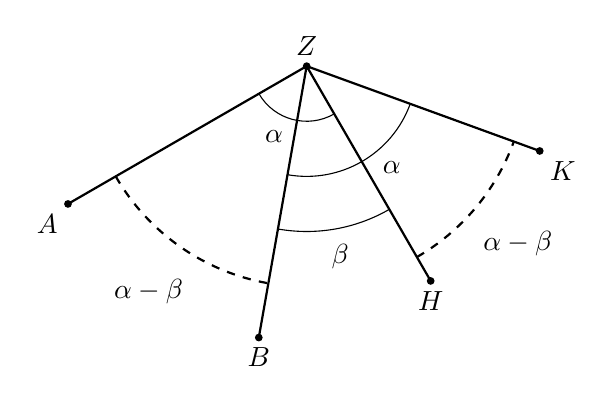
\begin{tikzpicture}[scale=.7]
\coordinate (Z) at (0,0);
\coordinate (A) at (-150:5cm);
\coordinate (B) at (-100:5cm);
\coordinate (H) at (-60:4.5cm);
\coordinate (K) at (-20:4.5cm);
\fill (Z) circle[radius=2pt];
\fill (A) circle[radius=2pt];
\fill (B) circle[radius=2pt];
\fill (H) circle[radius=2pt];
\fill (K) circle[radius=2pt];
\draw[thick] (A) node[below left] {$A$} -- (Z) node[above] {$Z$} -- (B) node[below] {$B$};
\draw[thick] (H) node[below] {$H$} -- (Z) -- (K) node[below right] {$K$};
\draw (-150:1cm) arc (-150:-60:1);
\draw (-100:2cm) arc (-100:-20:2);
\draw (-100:3cm) arc (-100:-60:3);
\draw[thick,dashed] (-150:4cm) arc (-150:-100:4);
\draw[thick,dashed] (-60:4cm) arc (-60:-20:4);
\node at (-115:1.4) {$\alpha$};
\node at (-50:2.4) {$\alpha$};
\node at (-80:3.5) {$\beta$};
\node at (-40:5) {$\alpha - \beta$};
\node at (-125:5) {$\alpha - \beta$};
\end{tikzpicture}
\vspace*{-10pt}
\end{center}
\end{quote}
and $\triangle ZAB$ and $\triangle ZHK$ are similar.

\begin{center}
\begin{tikzpicture}[scale=.45]
\coordinate (Z) at (0,0);
\coordinate (A) at (-130:5cm);
\coordinate (B) at (-90:5cm);
\fill (Z) node[above left] {$Z$} circle[radius=4pt];
\fill (A) node[below left] {$A$} circle[radius=3pt];
\fill (B) node[below] {$B$} circle[radius=3pt];
\draw[name path=c1] (Z) circle[radius=5cm];
\draw[name path=c2] (Z) circle[radius=2.5cm];
\node at (2,5) {$c_1$};
\node at (2,2.5) {$c_2$};
\draw[thick] (A) -- node[below,yshift=-6pt] {$s$} (B);
\path[thick,dashed] (A) -- +(20:120pt) coordinate (H);
\fill (H) node[below] {$H$} circle[radius=3pt];
\path[thick,dashed] (B) -- +(60:120pt) coordinate (K);
\fill (K) node[right] {$K$} circle[radius=3pt];
\draw[thick] (Z) -- node[left,xshift=-2pt,yshift=-2pt] {$m$} (A);
\draw[thick] (Z) -- (B);
\draw[thick] (Z) -- (H);
\draw[thick] (Z) -- node[above] {$n$} (K);
\draw[thick] (H) -- node[below right] {$x$} (K);
\draw[thick,dashed] (A) -- (H);
\draw[thick,dashed] (B) -- (K);
\end{tikzpicture}
\vspace*{-10pt}
\end{center}
Then $\frac{m}{s} = \frac{n}{x}$ and $x=\frac{n}{m}s$. 

%%%%%%%%%%%%%%%%%%%%%%%%%%%%%%%%%%%%%%%%%%%%%%%%%%%%%%%%%%%%%%%

Now for the solutions to I. and II. above.

\textbf{I’.} Find the point of intersection $S$ of two straight lines $AB$ and $CD$, each of which is given by two points, with compass alone.

\textbf{Solution.} Let $C'$ and $D'$ be reflections of $C$ and $D$ about line $AB$ respectively. The sought-for point of intersection $S$ then lies on line $C'D'$.

\begin{quote}
\vspace*{-8pt}
$CD$ and $C'D'$ intersect $AB$ at the same point $S$ because the reflection around $AB$ preserves distance: $C'S=CS$ and $D'S=DS$.
\end{quote}

\begin{center}
\begin{tikzpicture}[scale=.8]
\coordinate (A) at (-4,0);
\coordinate (B) at (2,0);
\coordinate (C) at (-3,2);
\coordinate (D) at (1,-1);
\coordinate (Cp) at (-3,-2);
\coordinate (Dp) at (1,1);
\fill (A) node[below] {$A$} circle[radius=2pt];
\fill (B) node[below] {$B$} circle[radius=2pt];
\fill (C) node[above] {$C$} circle[radius=2pt];
\fill (D) node[below] {$D$} circle[radius=2pt];
\fill (Cp) node[below] {$C'$} circle[radius=2pt];
\fill (Dp) node[above] {$D'$} circle[radius=2pt];
\draw[name path=ab] ($(A)!1.3!(B)$) -- ($(B)!1.3!(A)$);
\draw[name path=cd] ($(C)!1.2!(D)$) -- ($(D)!1.1!(C)$);
\path [name intersections={of=ab and cd,by={S}}];
\fill (S) node[above] {$S$} circle[radius=2pt];
\draw (Cp) -- (Dp);
\draw[thick,dashed] (C) -- node[above left] {$c$} (Cp);
\draw[thick,dashed] (D) -- node[above right] {$d$} (Dp);
\path (C) -- node[right,xshift=2pt] {$x$} (S);
\path (S) -- node[left,near end,xshift=-2pt] {$e-x$} (D);
\node at (-1,-2.5) {\mbox{\boldmath $CD=C'D'=e$}};
\end{tikzpicture}
\end{center}

$\triangle CSC'$ and $\triangle DSD'$ are similar so $\frac{CS}{DS} = \frac{CC'}{DD'}$. With $x = CS, c = CC', d = DD'$ and $e = CD$, we get $\frac{x}{e-x} = \frac{c}{d}$ or $x=\frac{c}{c+d}e$. (If $D$ is on the same side of $AB$ as $C$, then $x = \frac{c}{c-d}e$.)

\begin{quote}
\vspace*{-6pt}
Here is the diagram for $D$ on the same side of $AB$ as $C$:
\begin{center}
\begin{tikzpicture}[scale=.8]
\coordinate (A) at (-4,0);
\coordinate (B) at (2,0);
\coordinate (C) at (-3,2);
\coordinate (D) at (-1,1);
\coordinate (Cp) at (-3,-2);
\coordinate (Dp) at (-1,-1);
\fill (A) node[below] {$A$} circle[radius=2pt];
\fill (B) node[below] {$B$} circle[radius=2pt];
\fill (C) node[above] {$C$} circle[radius=2pt];
\fill (D) node[above] {$D$} circle[radius=2pt];
\fill (Cp) node[below] {$C'$} circle[radius=2pt];
\fill (Dp) node[below] {$D'$} circle[radius=2pt];
\draw[name path=ab] ($(A)!1.3!(B)$) -- ($(B)!1.3!(A)$);
\draw[name path=cd] ($(C)!2.2!(D)$) -- ($(D)!1.1!(C)$);
\path [name intersections={of=ab and cd,by={S}}];
\fill (S) node[above] {$S$} circle[radius=2pt];
\draw (Cp) -- (S);
\draw[thick,dashed] (C) -- node[above left] {$c$} (Cp);
\draw[thick,dashed] (D) -- node[above right] {$d$} (Dp);
\path (C) -- node[above] {$e$} (D);
\path (Cp) -- node[below] {$e$} (Dp);
\path (D) -- node[above right,xshift=-4pt] {$x-e$} (S);
\path (Dp) -- node[below right,xshift=-4pt] {$x-e$} (S);
\node at (1,-2.5) {\mbox{\boldmath $CS=C'S=x$}};
\end{tikzpicture}
\end{center}
 The similarity of the triangles $\triangle CSC'$ and $\triangle DSD'$ gives $\frac{x}{x-e}=\frac{c}{d}$ and we can solve for $x=\frac{c}{c-d}e$.
\end{quote}
$c + d = CH$ where $H$ is the intersection point of $c(C',d)$ and $c(D,e)$  on line $CC'$.

\begin{center}
\vspace*{-6pt}
\begin{tikzpicture}[scale=.8]
\coordinate (A) at (-4,0);
\coordinate (B) at (2,0);
\coordinate (C) at (-3,2);
\coordinate (D) at (1,-1);
\coordinate (Cp) at (-3,-2);
\coordinate (Dp) at (1,1);
\fill (A) node[below left] {$A$} circle[radius=2pt];
\fill (B) node[below] {$B$} circle[radius=2pt];
\fill (C) node[above] {$C$} circle[radius=2pt];
\fill (D) node[below] {$D$} circle[radius=2pt];
\fill (Cp) node[left] {$C'$} circle[radius=2pt];
\fill (Dp) node[above] {$D'$} circle[radius=2pt];
\draw[name path=ab] ($(A)!1.3!(B)$) -- ($(B)!1.3!(A)$);
\draw[name path=cd] ($(C)!1.2!(D)$) -- ($(D)!1.1!(C)$);
\path [name intersections={of=ab and cd,by={S}}];
\fill (S) node[above,yshift=4pt] {$S$} circle[radius=2pt];
\draw (Cp) -- node[below right] {$e$} (Dp);
\path (C) -- node[above left] {$c$} (Cp);
\draw[thick,dashed] (D) -- node[above right] {$d$} (Dp);
\node at (3,-3) {\mbox{\boldmath $CD=C'D'=DH=e$}};
\draw[name path=circled] (D) let
  \p1 = ($ (D) - (C) $),
  \n2 = {veclen(\x1,\y1)}
in
  ++(130:\n2) arc (130:230:\n2);

\draw[name path=circlecp] (Cp) let
  \p1 = ($ (D) - (Dp) $),
  \n2 = {veclen(\x1,\y1)}
in
  ++(-180:\n2) arc (-180:0:\n2);
\path [name intersections={of=circled and circlecp,by={H}}];
\fill (H) node[below left] {$H$} circle[radius=2pt];
\draw[thick,dashed] ($(C)!1.2!(H)$) -- (C);
\draw (H) -- node[right] {$d$} (Cp);
\draw (D) -- node[right,xshift=14pt,yshift=8pt] {$e$} (H);
\end{tikzpicture}
\vspace*{-10pt}
\end{center}

\begin{quote}
The circle $c(C',d)$ consists of the points at distance $d$ from $C'$. We claim that $H$, the intersection of $c(C',d)$ and $c(D,e)$, is on the extension of the line segment $CC'$, so that $CH$ is a line segment of length $CH=CC'+C'H=c+d$.

We previously defined $C'D' = e$ and $D'D=d$. The definition of $H$ as the intersection of the circles $c(C',d)$ and $c(D,e)$ gives $HC'=d$, $DH=e$. Therefore, the quadrilateral $C'D'DH$ is a parallelogram, since the lengths of both pairs of opposite sides are equal. $DD'$ was constructed so that it is parallel to $CC'$, so $C'H$, which is parallel to $DD'$ is also parallel to $C'$. Since one of its end points is $C'$, it must be on the line containing $CC'$, and the length of $CH$ is $c+d)$.
\end{quote}

($CH = c - d$ in case $D$ is on the same side of $AB$ as $C$.) Preliminary problem 4 then allows us to construct $x$, and from that $S$ as the intersection of arcs of the circles $c(C,x)$ and $c(C',x)$.

\begin{center}
\begin{tikzpicture}[scale=.8]
\coordinate (A) at (-4,0);
\coordinate (B) at (2,0);
\coordinate (C) at (-3,2);
\coordinate (D) at (1,-1);
\coordinate (Cp) at (-3,-2);
\coordinate (Dp) at (1,1);
\fill (A) node[below left] {$A$} circle[radius=2pt];
\fill (B) node[below] {$B$} circle[radius=2pt];
\fill (C) node[above] {$C$} circle[radius=2pt];
\fill (D) node[below] {$D$} circle[radius=2pt];
\fill (Cp) node[left] {$C'$} circle[radius=2pt];
\fill (Dp) node[above] {$D'$} circle[radius=2pt];
\draw[name path=ab] ($(A)!1.3!(B)$) -- ($(B)!1.3!(A)$);
\draw[name path=cd] ($(C)!1.2!(D)$) -- ($(D)!1.1!(C)$);
\path [name intersections={of=ab and cd,by={S}}];
\fill (S) node[above,yshift=4pt] {$S$} circle[radius=2pt];
\draw (Cp) -- (Dp);
\path (C) -- node[above,yshift=4pt] {$x$} (S);
\path (Cp) -- node[below,yshift=-4pt] {$x$} (S);
\path (C) -- node[above left] {$c$} (Cp);
\draw[thick,dashed] (D) -- node[above right] {$d$} (Dp);
\node at (2.5,-3) {\mbox{\boldmath $CD=C'D'=DH=e$}};
\draw[name path=circled] (C) let
  \p1 = ($ (S) - (C) $),
  \n2 = {veclen(\x1,\y1)}
in
  ++(-10:\n2) arc (-10:-100:\n2);

\draw[name path=circlecp] (Cp) let
  \p1 = ($ (S) - (C) $),
  \n2 = {veclen(\x1,\y1)}
in
  ++(100:\n2) arc (100:0:\n2);
\draw[thick,dashed] (Cp) -- (C);
\end{tikzpicture}
\vspace*{-8pt}
\end{center}


\begin{quote}
$x$ is the length of $CS$ which equals the length of $C'S$ because reflection preserves distances, so all we have to do is compute $x$, and then $S$ will be the intersection of the circles $c(C,x), c(C',x)$. By Preliminary problem 4, we can compute $x=\frac{c}{c+d}e$ given $c,e,d$, where the line segment of length $c+d$ is constructed above as $CH$.
\end{quote}

%%%%%%%%%%%%%%%%%%%%%%%%%%%%%%%%%%%%%%%%%%%%%%%%%%%%%%%%%%%%%%%

\textbf{II’.} Determine the point of intersection $S$ of a given circle $k$ and a given straight line $AB$ with compass alone.

\textbf{Solution.} Let $k = c(M,r)$, and $M'$ be the reflection of $M$ about line $AB$.

\begin{quote}
\vspace*{-10pt}
Recall from Prelim. problem 1 that a reflection can be constructed with compass alone given the points $A,B$ defining a line.
\end{quote}

\begin{center}
\vspace*{-10pt}
\begin{tikzpicture}[scale=.5]
\coordinate (A) at (-7,0);
\coordinate (B) at (8,0);
\coordinate (M) at (0,-2);
\coordinate (Mp) at (0,2);
\fill (A) node[below] {$A$} circle[radius=3pt];
\fill (B) node[below] {$B$} circle[radius=3pt];
\fill (M) node[below left] {$M$} circle[radius=3pt];
\fill (Mp) node[above left] {$M'$} circle[radius=2pt];
\draw[name path=c1] (M) circle[radius=3cm];
\draw[name path=c2] (Mp) circle[radius=3cm];
\draw[name path=ab] ($(A)!1.2!(B)$) -- ($(B)!1.2!(A)$);
\path [name intersections={of=c1 and c2,by={S1,S2}}];
\fill (S1) circle[radius=3pt];
\fill (S2) circle[radius=3pt];
\path[name path=radius1] (M) -- ++(15:4cm);
\path [name intersections={of=c1 and radius1,by={R1}}];
\draw[thick,dashed] (M) -- node[below] {$r$} (R1);
\path[name path=radius2] (Mp) -- ++(40:4cm);
\path [name intersections={of=c2 and radius2,by={R2}}];
\draw[thick,dashed] (Mp) -- node[above] {$r$} (R2);
\fill (R1) circle[radius=3pt];
\fill (R2) circle[radius=3pt];
\end{tikzpicture}
\vspace*{-10pt}
\end{center}

The points of intersection are the points where $c(M,r)$ and $c(M',r)$ intersect. This construction cannot be done if $M$ is on line $AB$.

\begin{center}
\vspace*{-10pt}
\begin{tikzpicture}[scale=.5]
\coordinate (A) at (-7,0);
\coordinate (B) at (8,0);
\coordinate (M) at (0,0);
\fill (A) node[below] {$A$} circle[radius=3pt];
\fill (B) node[below] {$B$} circle[radius=3pt];
\fill (M) node[below left] {$M$} circle[radius=3pt];
\draw[name path=c1] (M) circle[radius=3cm];
\draw[name path=ab] ($(A)!1.2!(B)$) -- ($(B)!1.2!(A)$);
\path[name path=radius1] (M) -- ++(-30:4cm);
\path [name intersections={of=c1 and radius1,by={R1}}];
\draw[thick,dashed] (M) -- node[below] {$r$} (R1);
\path [name intersections={of=c1 and ab,by={S1,S2}}];
\fill (S1) node[above right] {$AM+r$} circle[radius=3pt];
\fill (S2) node[above left] {$AM-r$} circle[radius=3pt];
\fill (R1) circle[radius=3pt];
\end{tikzpicture}
\vspace*{-10pt}
\end{center}
In this exceptional case, extend and shorten $AM$ by $r$ by Prelim 3; the end points of the extended and shortened segments are the desired points. 

